L’objectif de ce rapport et de présenter d’une manière claire le fonctionnement de l'application
réalisée au cours de mon stage d’été. En premier lieu j'ai commencé par
une étude de l’existant avec une critique afin d'éviter les erreurs au cours du
projet.

Cette étude m'a permis de concevoir les besoins fonctionnels et non fonctionnels, puis passer
à l’étape de conception, qui, dans laquelle j'ai schématisé mon travail sous forme des diagrammes pour faciliter la compréhension et mieux décrire l'application.
Enfin j'ai réalisé l'application tout en respectant les exigences soulignées lors de
la conception. Certes, deux mois ne sont pas suffisants pour compléter un grand projet comme ceci, pourtant la partie la plus difficile et la plus complexe a été réalisée et a été appréciée par mon encadrant.

En effet, la partie reporting, que j’ai n’est pas pu terminé, a fini par la création du modèle pour le traitement des données dans PowerBI suivant:
\begin{figure}[H]
    \begin{center}
        \fbox{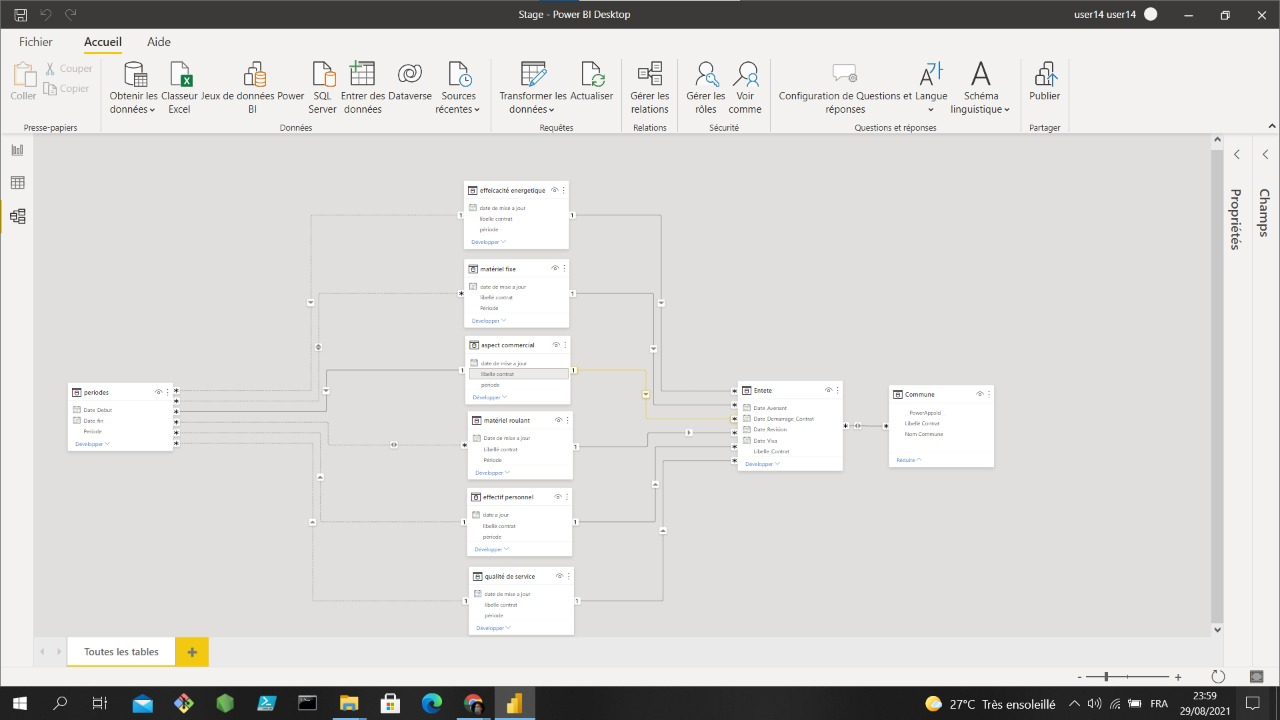
\includegraphics[scale=0.40]{PowerBi.jpeg}}
        \caption{Modèle des données en PowerBI }
    \end{center}
\end{figure}

Au terme de ce travail, je peux affirmer que ce stage a été plein d’intérêt et d'apprentissage. D'ailleurs, j'ai pu travailler sur des nouveaux logiciels.
En addition, j'ai pu vraiment découvrir le déroulement de la vie professionnelle à travers des réunions avec mon encadrant et les autres membres de l’entreprise.
J'ai appris comment une équipe travaille pour réussir un projet. Ceci m'a donné une idée sur les situations que je vais confronter au futur proche en tant qu'ingénieur en génie logiciel.
